\section{Data Processing Package - Structure}

Each data processing package has four folders (Input-files, Output-files, Scripts-functions, Log-files) and one file (run.sh). We can change the whole package name and transfer it to other location in memory, or other computers. Once we pick a name to the internal folders, we can't change the name of folders, because of using these names for handling the path. Each file and folder has specific functionality.

\begin{figure} [ht]
\centering
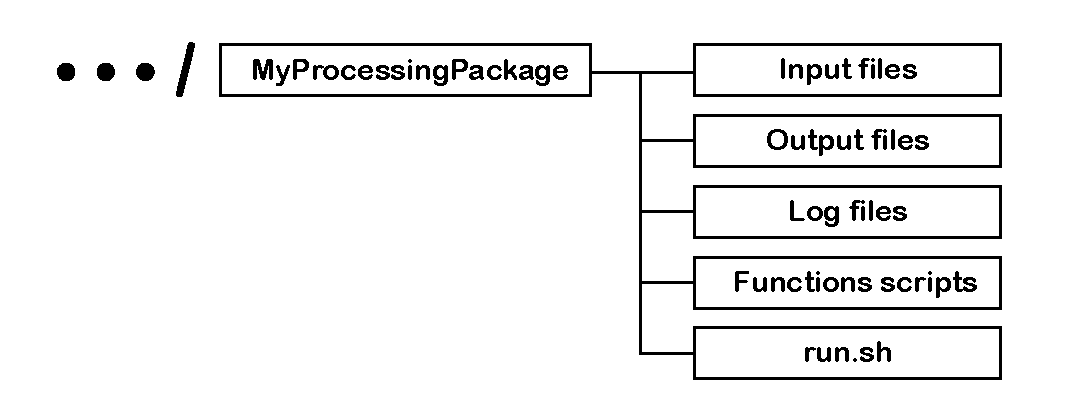
\includegraphics[scale=0.6]{figures/pdf/Figure02.pdf} 
\caption{File and folders of the data processing package.}
\label{fig:structure}
\end{figure}


\textbf{Input-files} folder involves all files (or folders) that we want to process them. These files can be a raw data, or list of file names, or results of other project to merge with our results.\textbf{Output-files} folder involves all files that we want to produce, it could be a text files, figures, pdf files, and temporary files. \textbf{Log-files} folder involves files that we want to track the program's operation. It could be the history of runs (like, who ran the program and when), report the success and failure for each set of data, and summary of the processing.  \textbf{Scripts-functions} has all functions and scripts of Matlab and Shell (or other programing languages). We make sure that never add or delete or modify any data in this folder. \textbf{run.sh} is a shell script file that includes the whole processing sequence. Basically this file calls the other scripts. This file is a place to define different parameters to expand the functionality of the processing package. For example you can ask the program to keep data of all steps, or only report a final pdf file, or ignore some steps. 


\section{Handling the path}

The most important factor in writing a processing package is handling the path. In each step of programming, we need to know, where are we (in terms of computer path), and where we want to be. Where is the input data and where we need to print out the output data. We accept the following axioms:

\begin{itemize}
  \item We can run any program, script, function in the memory, if we know the location of the program.
  \item We can load any data, into the program, if we know the location of the data.
  \item We can write any data, in any part of memory, if we know the destination path. 
\end{itemize}

Since we run the \textbf{run.sh}, the program has access to the current path (using $pwd$). So we can navigate to other folders (since we know the folder names) through adding the folder name to the current path. 

\begin{figure} [ht]
\centering
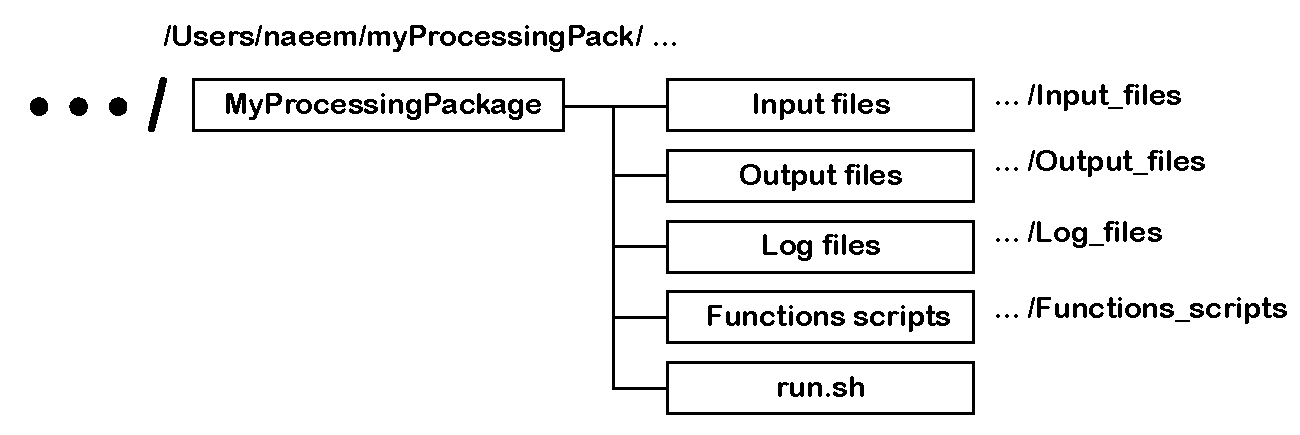
\includegraphics[scale=0.6]{figures/pdf/Figure03.pdf} 
\caption{Relative path of folders.}
\label{fig:structure}
\end{figure}


\section{Basic Shell Commands}

Here is the list of important Shell commands for the project, you may need other commands depending on the complication of the project. There are many resources to learn how to write a shell scripts. 





\begin{table}[h]

\begin{tabular}{ c  m{12cm} }
 \textbf{mkdir}          & make a directory  \\ 
 \end{tabular}
\label{tab:b_k_m_param}
\end{table}